\section{Kernel Discriminant Analysis against Masking}

\begin{frame}
\frametitle{Contents}
\begin{itemize}
\item \textcolor{grey}{Introduction to LDA: as a classifier, and as a feature extractor}
\item \important{Introduction to masking countermeasure and Kernel Discriminant Analysis as a feature extractor}
\item Convolutional Neural Networks and Data Augmentation to attack jitter-based countermeasure
\end{itemize}
\end{frame}

\begin{frame}
\frametitle{Dimensionality reduction in presence of sharing}
%\begin{block}{Countermeasures}
%Techniques to thwart side-channel attacks. 
%\begin{itemize}
%\item Hiding (\emph{ex:} random delay, shuffling, ...)
%\item Sharing  $\textcolor{red}{\longleftarrow}$ \textcolor{red}{makes selecting and projecting techniques ineffective}
%\end{itemize}
%\end{block}

\begin{block}{$(d-1)$th-order Sharing (or Masking)}
$Z$ split into shares  $Z = M_1 \star \dots \star M_d$ \\
with $M_1, \dots , M_{d-1}$ random shares (or masks) and $M_d = Z \star M_1^{-1}\star \dots \star M_{d-1}^{-1}$ \\
Shares are handled at different time samples $t_1,\dots, t_d$ so that each time sample is independent from $Z$: $f(Z) = \esper[\XXX\lvert Z]$ is constant.
\end{block}
\pause
\begin{block}{Higher-Order SCAs}
Exploit $f(Z) = \esper[\XXX[t_1]\XXX[t_2]\dots\XXX[t_d]\lvert Z]$ non-constant.\\
 
The statistic extracted from measurements, viewed as a multivariate polynomial in the time samples coordinates, must contain the $d$th-degree monomial $\XXX[t_1]\XXX[t_2]\dots\XXX[t_d]$.
\end{block}

\end{frame}

\begin{frame}
\frametitle{PoIs Research}
How to detect the $d$-tuple $t_1,\dots, t_d$? 
\begin{block}{A lacking literature}
\begin{itemize}
\item many HO attacks papers assume the knowledge of $t_1,\dots, t_d$
\item PoI research exploiting the random shares knowledge (back to unprotected case using $M_1,\dots , M_d$ instead of $Z$)
\item naive strategy: infer over all possible $d$-tuples 
\item Hand selection via educated guess \cite{Oswald2006}
\end{itemize}
\end{block}

\begin{block}{Generalizing extractors for higher-order context}
\begin{itemize}
\item Selecting extractors $\longrightarrow$ Projection Pursuits \cite{PP}
\item Projecting extractors $\longrightarrow$ Kernel Discriminant Analysis [CARDIS '16]
\end{itemize}
\end{block}
\end{frame}

\subsection{Kernel Discriminant Analysis}
\begin{frame}
[fragile]
\frametitle{Kernel Discriminant Analysis (KDA) [to appear at CARDIS '16]}
\vspace{-10pt}
\begin{figure}
\centering
{
\begin{tikzpicture}
\matrix (m) [matrix of math nodes, row sep=3em,
column sep=3em, text height=1.5ex, text depth=0.25ex]
{ \mathbb{R}^\traceLength & \featureSpace & \mathbb{R}^\newTraceLength \\ };
\path[->]
(m-1-1) edge node[above] {$\Phi$} (m-1-2);
         %edge [bend left=30] (m-2-2)
         %edge [bend right=15] (m-2-2);
\path[->]
($(m-1-2.north east)-(0,0.1)$) edge node[above] {$\extract^{\mathrm{PCA}}$} ($(m-1-3.north west)-(0,0.1)$);
\path[->]
($(m-1-2.south east)+(0,0.15)$) edge node[below] {$\extract^{\mathrm{LDA}}$} ($(m-1-3.south west)+(0,0.15)$);

\path[->]
(m-1-1) edge [bend left=50] node[above] {$\extract^{\mathrm{KPCA}}$} (m-1-3)
(m-1-1) edge [bend right=50] node[below] {$\extract^{\mathrm{KDA}}$} (m-1-3);

\end{tikzpicture} 
}
\end{figure}
\vspace{-10pt}
$\mathcal{F}$ contains all $d$-th degree monomials \small{(dimension increases combinatorially: ${{D}\choose{d}}$)}
\pause

\begin{block}{Kernel function}
 \begin{centering}$K\colon\mathbb{R}^D\times \mathbb{R}^D \rightarrow \mathbb{R} \qquad K(\sss[]{i},\sss[]{j}) = \Phi(\sss[]{i})\cdot \Phi(\sss[]{j})
$\end{centering}
\end{block}
\pause
\vspace{-5pt}
\begin{block}{Polynomial kernel function}
dth-degree polynomial kernel: $K\colon(\sss[]{i},\sss[]{j}) \mapsto ( \sss[]{i}\cdot \sss[]{j})^d \leftrightarrow$  all $d$-th degree monomials ($\mathcal{F}$).
\pause

Example: 
$d=2, D=2$; $\sss[]{i} = [a,b]$ , $\sss[]{j} = [c,d]$ $\longrightarrow$
\vspace{-10pt}
\begin{equation*}
\textcolor{olive}{K(\sss[]{i},\sss[]{j})} = (ac + bd)^2 = a^2c^2 + 2abcd + b^2d^2 \mbox{ ,}
\end{equation*}

%\begin{align}
%&\Phi \colon \mathbb{R}^2 \rightarrow \mathbb{R}^3\\
%&\Phi \colon [a,b]\mapsto [a^2, \sqrt{2}ab, b^2]\\
%&\Phi \colon [c,d]\mapsto [c^2, \sqrt{2}cd, d^2].
%\end{align}
\vspace{-15pt}
\begin{equation*}
K \longleftrightarrow \Phi\colon \Bbb{R}^2\rightarrow\Bbb{R}^3 \qquad \Phi(u,v) =  [u^2, \sqrt{2}uv, v^2]
\end{equation*}
$\textcolor{olive}{\Phi(\sss[]{i})\cdot \Phi(\sss[]{j})} = a^2c^2 + 2abcd + b^2d^2 = K(\sss[]{i},\sss[]{j})$

\end{block}
\end{frame}

\begin{frame}
[fragile]
\frametitle{LDA to KDA}
\vspace{-30pt}
\begin{figure}
\centering
{
\begin{tikzpicture}
\matrix (m) [matrix of math nodes, row sep=3em,
column sep=3em, text height=1.5ex, text depth=0.25ex]
{ \mathbb{R}^\traceLength & \featureSpace & \mathbb{R}^\newTraceLength \\ };
\path[->]
(m-1-1) edge node[above] {$\Phi$} (m-1-2);
         %edge [bend left=30] (m-2-2)
         %edge [bend right=15] (m-2-2);
\path[->]
($(m-1-2.north east)-(0,0.1)$) edge node[above] {$\extract^{\mathrm{PCA}}$} ($(m-1-3.north west)-(0,0.1)$);
\path[->]
($(m-1-2.south east)+(0,0.15)$) edge node[below] {$\extract^{\mathrm{LDA}}$} ($(m-1-3.south west)+(0,0.15)$);

\path[->]
(m-1-1) edge [bend left=50] node[above] {$\extract^{\mathrm{KPCA}}$} (m-1-3)
(m-1-1) edge [bend right=50] node[below] {$\extract^{\mathrm{KDA}}$} (m-1-3);

\end{tikzpicture} 
}
\end{figure}
\vspace{-15pt}
\begin{columns}
\begin{column}{.5\textwidth}
\begin{block}{LDA}
\begin{itemize}
\item $\AAlpha_i$ eigenvectors of $\SW^{-1}\SB$
\item $\SB$ and $\SW$ depend on data $(\sss[z_i]{i})$ [$D\times D$]
\item $\extract^{LDA}_{\ell}(\xxx) = \sum_{i=1}^D \AAlpha_{\ell}[i]\xxx[i] $
\end{itemize}
\end{block}
\end{column}

\begin{column}{.5\textwidth}
\begin{block}{KDA}
\begin{itemize}
\item $\nununu_i$ eigenvectors of $(\SW^K)^{-1}\SB^K$
\item $\SB^K$ and $\SW^K$ depend on kernel function images $K(\sss[z_i]{i}, \sss[z_j]{j})$ [$N\times N$]
\item $\extract^{\mathrm{KDA}}_{\ell}(\vec{x}) = \sum_{i=1}^{\NPoI}\nununu_\ell[i]K(\sss[z_i]{i}, \sss[]{}) $
\end{itemize}
\end{block}
\end{column}
\end{columns}
\vspace{-5pt}
\begin{block}{Application Issues}
\begin{itemize}
\item regularization : $\SW^K \leftarrow \SW^K + \mu \III$
\item computational complexity is $O(N^3)$ 
\item non-injective model $\sensVarSet \rightarrow m(\sensVarSet)$ to reduce the number of classes (to improve KDA accuracy in detecting class separating subspaces)
\item asymmetric 'KDA/profiling' approach (to improve profiling accuracy)
\end{itemize}
\end{block}

\end{frame}

\subsection{Experimental Results}


\begin{frame}
\frametitle{Experimental results}
\begin{itemize}
\item $D = 200$: length of rough trace (interesting clock cycles selected)
\item $d=2$, feature extracted from a $200^2 = 40.000$-sized space
\item $d=3 \rightarrow 200^3=6.000.000$ , $d=4 \rightarrow 200^4 = 800.000.000$
\end{itemize}
\begin{figure}[t]

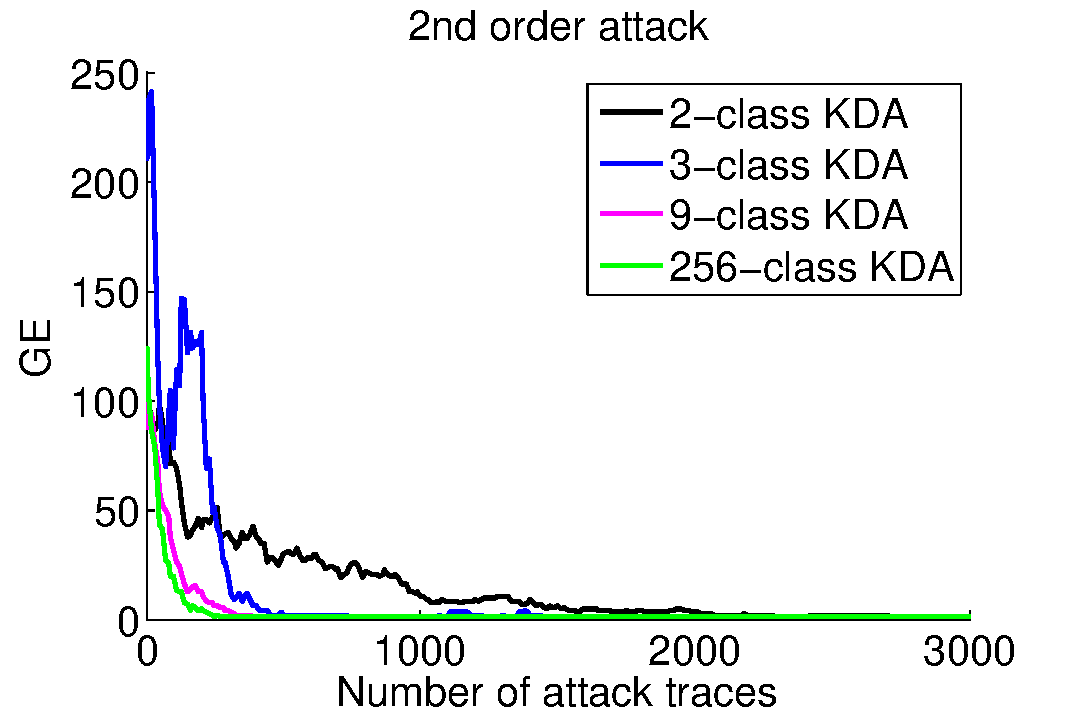
\includegraphics[width=.4\textwidth]{figures/2order_classes_TA.pdf}
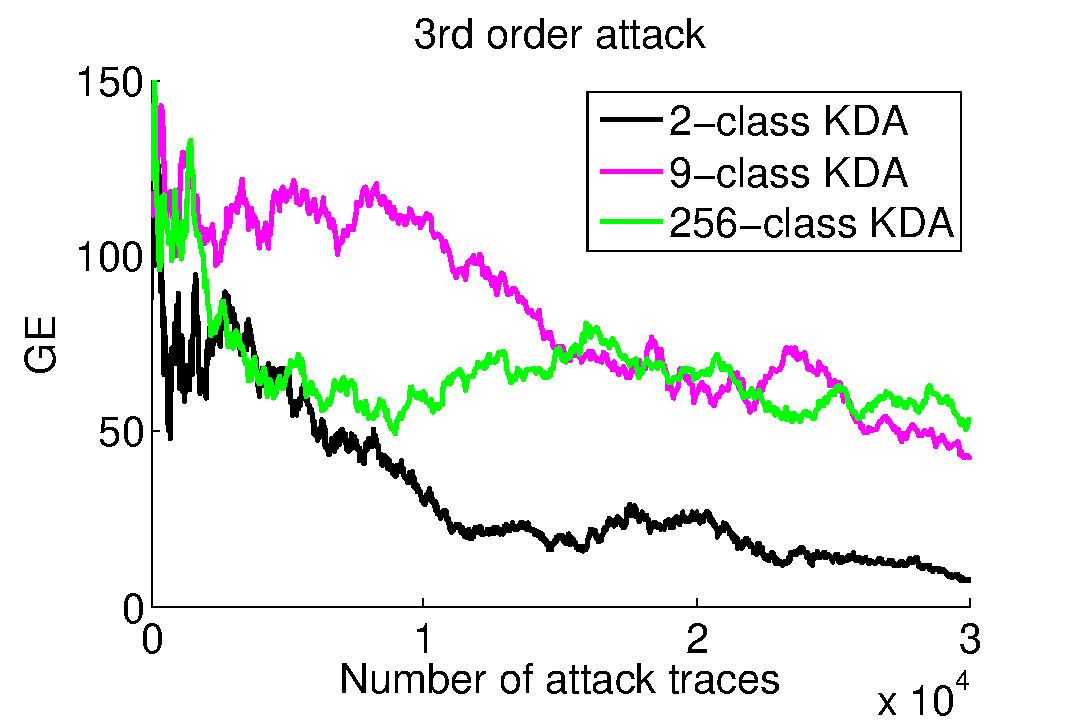
\includegraphics[width=.4\textwidth]{figures/3order_new.pdf}
\end{figure}
\vspace{-10pt}
\begin{figure}[t]

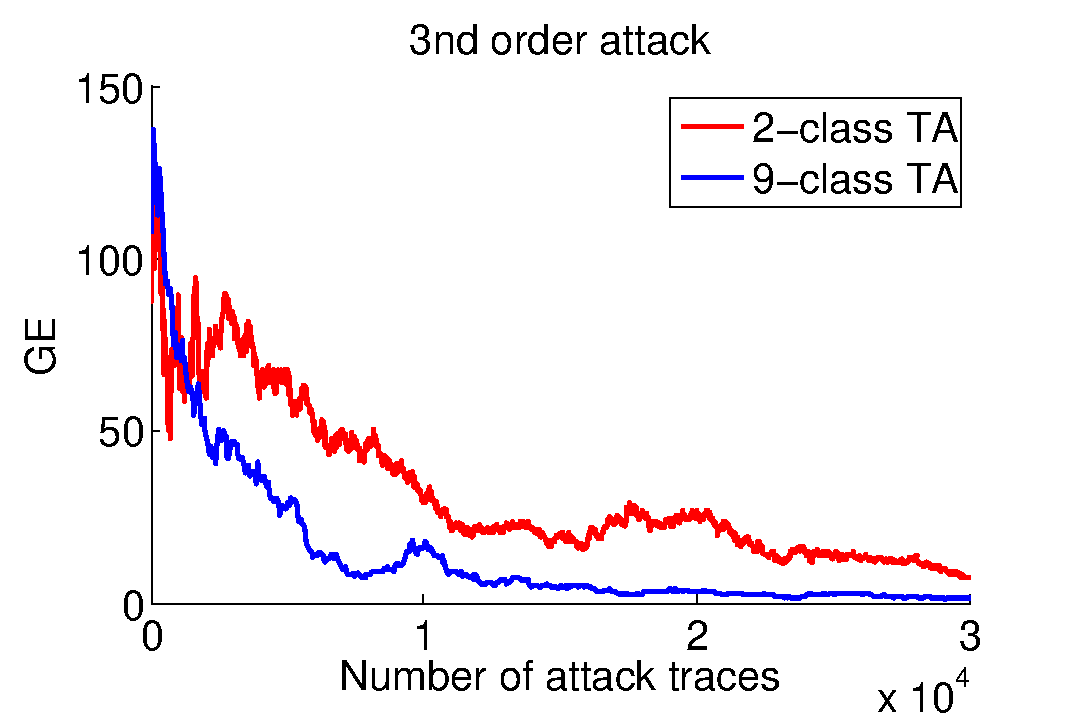
\includegraphics[width=.4\textwidth]{figures/3order_2_9.pdf}
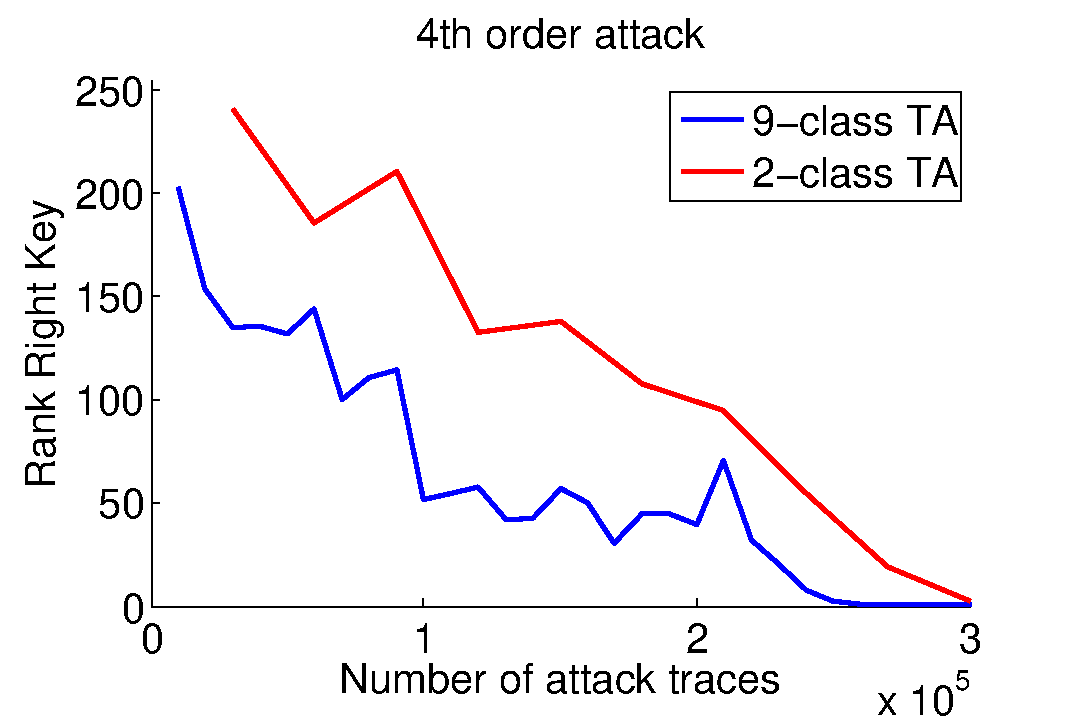
\includegraphics[width=.4\textwidth]{figures/4order_2_9.pdf}
\end{figure}
\end{frame}